\documentclass{article}
\usepackage{graphicx} % Required for inserting images
\usepackage{amsmath, amssymb, amsthm} 
%Allows to use of all the mathematics, equations, and symbols
\usepackage[letterpaper, top=1in, bottom=1.0in, left=1.2in, right=1.2in, heightrounded]{geometry}
\usepackage{graphicx, float}
%Packages for using images
\graphicspath{{Images/}}

\title{Artificial Intelligence (AI)}
\author{Suhyeon Kim}
\date{September 2025}

\begin{document}

\maketitle

\section{Vocabulary}
\subsection{Machine Learning}
System learn from data to identify patterns and make predictions or decisions with minimal human intervention

\subsection{Deep Learning}
A subset of machine learning that uses a multi-layered artificial neural networks to automatically learn complex patterns from large datasets. 

\subsection{Model}
A program that learns from data to find patterns and make predictions or decisions about new, unseen data without explicit human instruction. It is the output of a machine learning algorithm after it has been trained on a large dataset. 

\subsection{Channel}
A distinct feature or piece of information within a multi-dimensional dataset, particularly in CNNs, where an \underline{image is described by channels (like red, green, blue)} and output channels represent extracted features
\\
\\
- \textbf{Image Classification}: Classify the entire image into one of the classes. 

\noindent - \textbf{Image Classification with Localization}: Also, find the location of that object 

\noindent - \textbf{Object Detection}: Drawing bounding boxes around the object

\noindent - \textbf{Image Segmentation}: Classifying each of the pixels into the class

\subsection{Convolutional Neural Networks(CNN)}
Specialized in pattern recognition. Filters perform the pattern recognition. 

\begin{figure}[H]
    \centering
    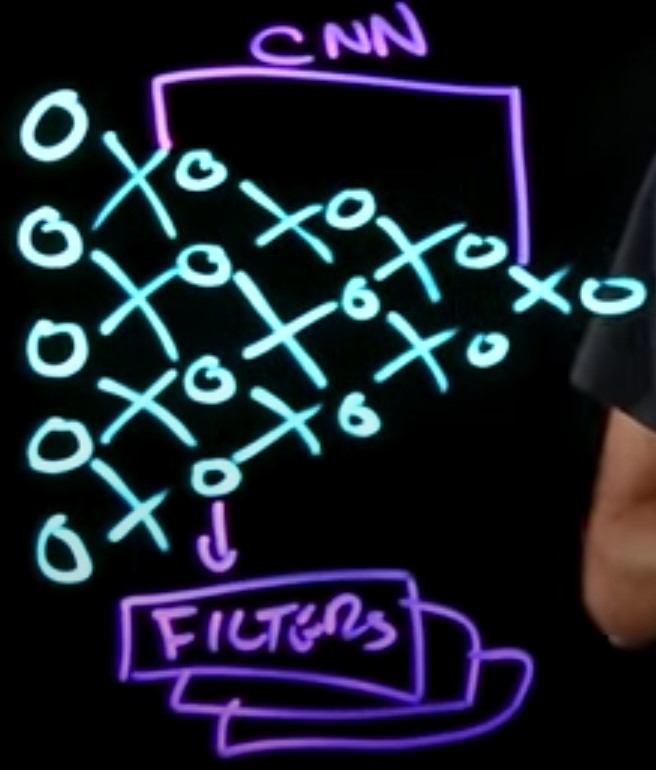
\includegraphics[width=0.3\linewidth]{1.jpg}
    \caption{Visualization of CNN}
    \label{fig:placeholder}
\end{figure}

\subsubsection{Filters}
An image can be transformed into pixels, which might be look similar to a 2D-array. Filter is a 3x3 array that shows a specific pattern. Then you compare this filter to an image and score how similar they are, and record the data into an array. Repeat this process until you cover the entire image. There are many filters, so repeat this process for each filter. This is the first layer of filters (Dot = Filter). As you go deeper, filters get abstracted, so the second filter might be an entired object you are looking for. Example, first filter = a line of left part of window, second filter = a window.  

\subsection{Type of Data}
\textbf{Training data}: Used to teach a machine learning model to recognize patterns 
\\
\\
\textbf{Validation data}: Used to tune the model's hyperparameters and evaluate its performance on unseen data during the training process to prevent overfitting 
\\
\\
\textbf{Hyperparameter}: A Configurable setting in machine learning that controls the learning process and model complexity

\subsection{Pipeline}
Workflow that chains together the sequential steps required to build, train, and deploy a machine learning model.

\begin{figure}[H]
    \centering
    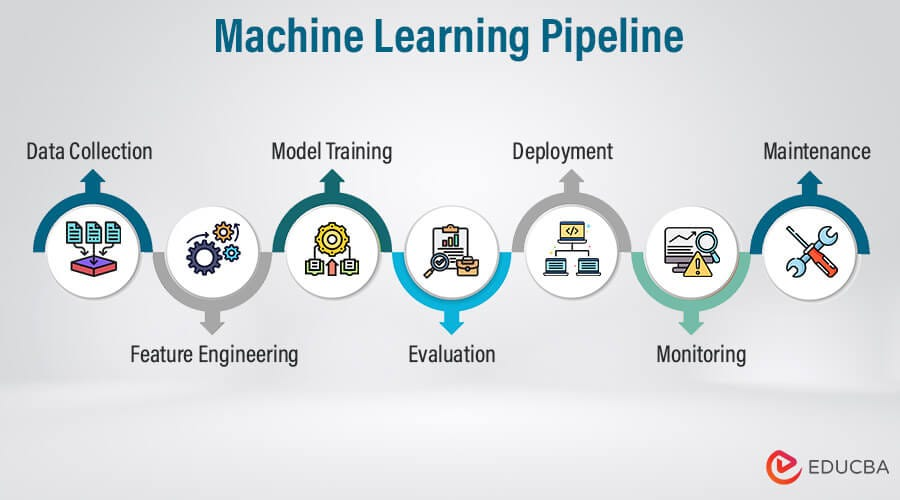
\includegraphics[width=0.3\linewidth]{2.jpg}
    \caption{Definition of Pipeline in machine learning}
    \label{fig:placeholder}
\end{figure}

\section{Building a Deep CNN Image Classifier}
\subsection{Dependencies(open-source framework)}
- \textbf{Tensorflow Tensorflow-gpu}: is an open-source machine learning framework that can leverage Graphics Processing Units (GPUs) for \underline{accelerated computation}, especially in deep learning tasks. Utilizing a GPU significantly speeds up model training and inference compared to using only a CPU.
\\
\\
- \textbf{opencv-python}: To remove dodgy images


\end{document}
